\section{Evaluation}
\label{sec:evaluation}


\begin{figure*}
  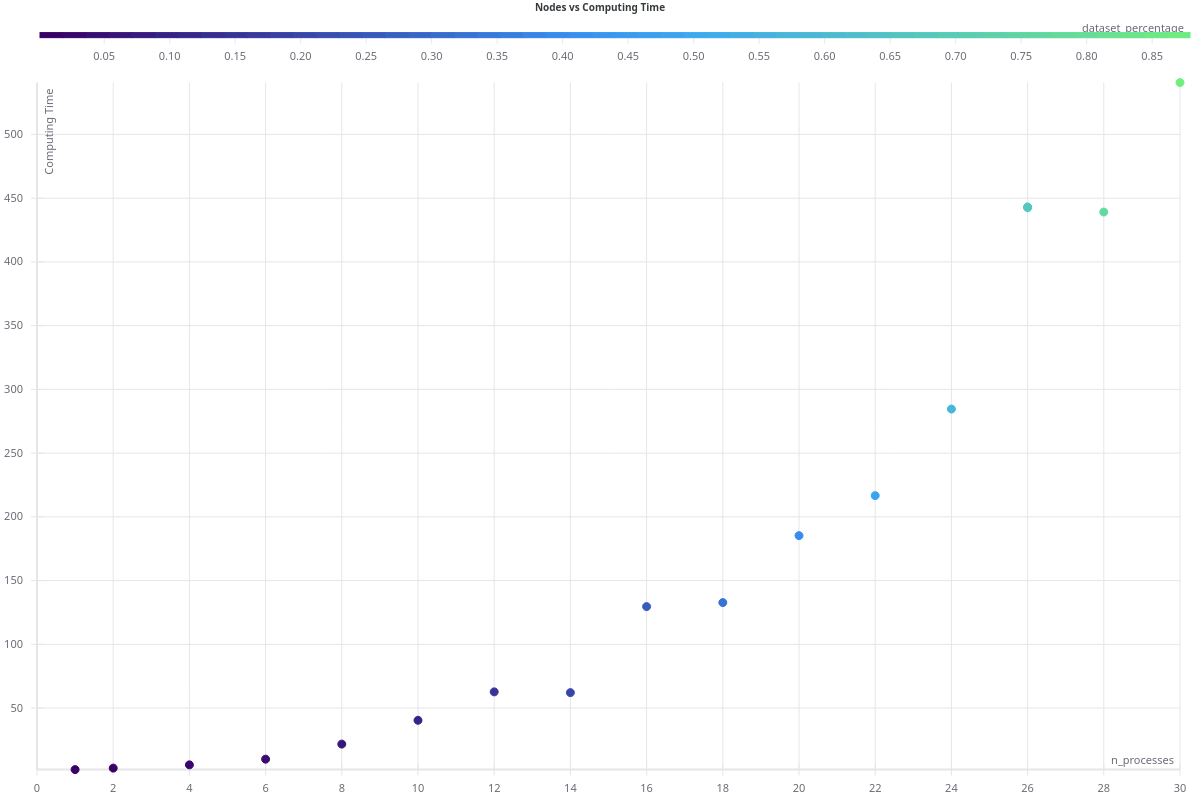
\includegraphics[width=0.9\linewidth]{images/weak_scaling_chart.png}
  \caption{Weak scaling behaviour of the spectral clustering algorithm.}\label{fig:weak_scaling}
\end{figure*}


\subsection{Strong Scaling}
\label{subsec:strong_scaling}


The first evaluation consisted in the strong scaling behaviour of the \gls{HeAT} implementation.
For this the same percentage of the dataset was used for all numbers of nodes.
The configuration was set to fixed 40\% of the Sentinel-1 dataset.
For the graph calcuation the fully connected graph was choosen. For an explanation of the graph type see \cref{subsec:spectral_clustering}.
Each node is assigned 90GB of \gls{RAM} and run in exclusive mode to keep the runtimes clean of the influence of other running programs.
All nodes run only 1 \gls{MPI} process and use the \gls{PyTorch} threading.

The results of the measurement can be seen in \cref{fig:strong_scaling}. As a baseline the same task was performed on 1 node and yielded a runtime of \(6489s\).
No nodes between \(2\) and \(10\) could be run for the profiling due to the message size limitation of \gls{MPI}. This is one of the current weak points
of \gls{HeAT} that will be fixed in the future.
But finding a workaround for the message limit takes a lot of time and effort.
Therefore, the graph only shows node runtimes above \(10\) nodes.

Interestingly the strong scaling performance is close to optimal and sometimes (e.g. 14-28 and 1-10) even better.
This seems due to 14 nodes performing worse than other configurations.
The same can be suspected for the \(1\) node baseline, which performed consistenly worse than the \(10x\) runtime of the \(10\) node configuration.

\subsection{Weak Scaling}
\label{subsec:weak_scaling}

For testing of the weak scaling the load per node should stay constant. Therefore, we fixed the
maximum number of nodes to 32.
The maximum number of nodes work on the full dataset. All smaller number of nodes work on the corresponding
percentage of the dataset in relation to the maximum number of nodes. When calculating the percentage, the runtime
of the choosen algorithm has to be considered. Since spectral clustering is in the runtime of \(O(n^2)\) with \(n\) samples,
we need to scale the fraction of the dataset squared as well:
\[percentage\_dataset = \left(\frac{nodes}{nodes_{max}}\right)^2\]

All other parameters stayed the same as in the strong scaling case.
The results of this profiling can be seen in \cref{fig:weak_scaling}.

In contrast to the strong scaling \cref{subsec:strong_scaling}, the weak scaling is not optimal. If the algorithm would scale perfectly, the runtime should be a
constant line, since the load stayed constant across all nodes. But the runtime seems to scale in \(O(n^2)\) when increasing the number of nodes.
This is probably due to the communication overhead when calculating the matrix multiplication.
Since the overall amount of data increases and the number of nodes increases which need to send the data between them, this seems the best explanation.

The increase in time could therfore be decreased by using faster communication. Since the available cluster has only one configured type of communication
this would need to be confirmed in further works.


\subsection{Clustering Results}
\label{subsec:clustering_results}

\begin{table}
    \centering
    \begin{tabular}{lll}
      \toprule
      Metric     &  ARI & V-Measure \\
      \midrule
      Training   &  -0.00005692  &  0.0001602     \\
      Validation &   & \\
      \bottomrule
    \end{tabular}
    \caption{The calculated metrics of the clustering result.}
    \label{tab:clustering_results}
  \end{table}

  \begin{figure*}
    \centering
    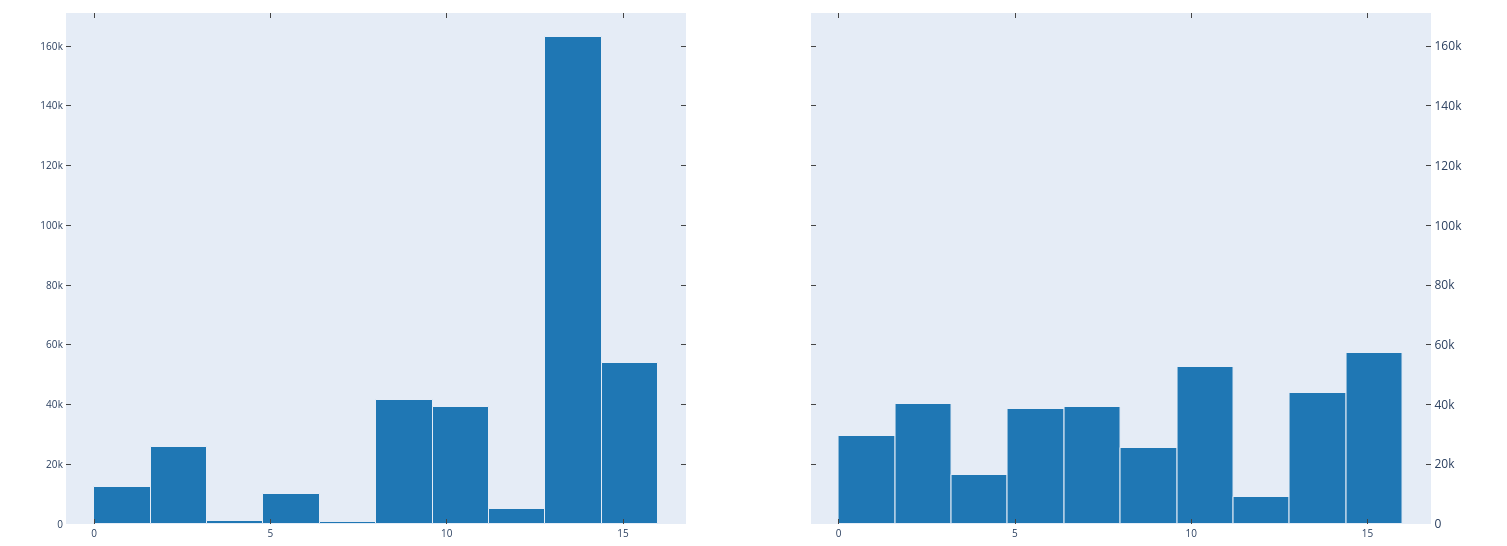
\includegraphics[width=0.9\linewidth]{images/label_distribution.png}
    \caption{Comparison of the label distribution with the original label distribution.}
    \label{fig:label_distribution}
  \end{figure*}

  \begin{figure}
    \centering
    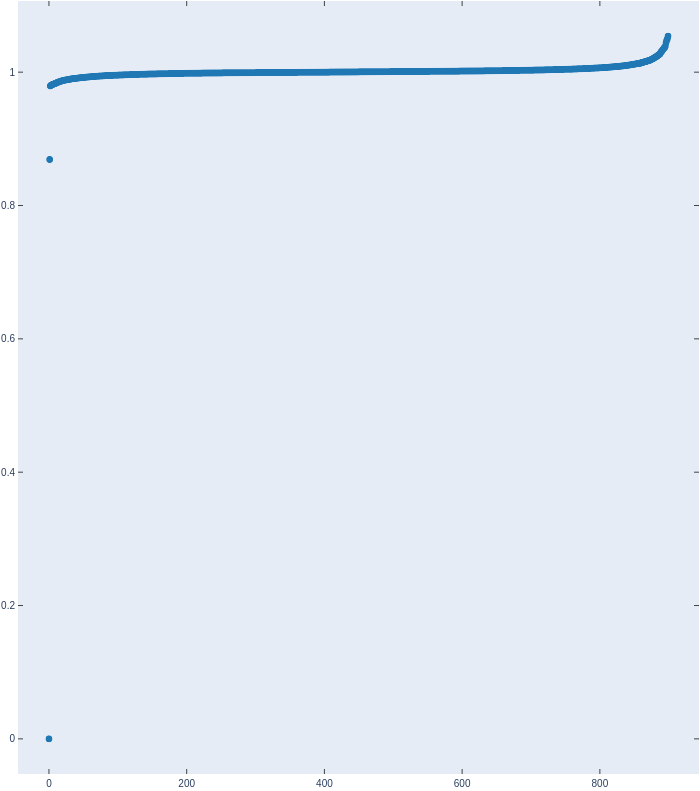
\includegraphics[width=0.9\linewidth]{images/eigenvalues.png}
    \caption{Sorted smallest 50 eigenvalues of the spectral clustering.}
    \label{fig:eigenvalues}
  \end{figure}



Although, the main focus of this work is the scaling behaviour of the implementation the results will be evaluated as
well. To evaluate the results metrics were presented in \cref{subsec:clustering_evaluation_metrics}.
They are calculated for the whole dataset and shown in \cref{tab:clustering_results}.
All metrics are close to \(0\) which indicates a random distribution of the labels with no correlation to the target
labels.

To confirm this, a plot of the predicted label distribution can be seen in \cref{fig:label_distribution}.
The labels do not match in any counts to the original labels. Therefore, they do not line up with the external labels
in the pairwise metrics.

The poor performance of the clustering can be due to a variety of reasons.
First, the \gls{LCZ} have been desinged on paper and were not extracted from data. Therefore, it is unlikely that
the zones would all line up with any structure in the data itself.
But, especially the land types could have been expected to line up with the zone specification.

When taking a look at the eigenvalue spectrum in \cref{fig:eigenvalues} most of the eigenvalues seem very close together and
further explain the poor performance. The biggest gap in the eigenvalues is located at eigenvalue 3. This so called spectral gap
implies 3 found clusters with spectral clustering. Which are found using the spectral gap implementation in \gls{HeAT} as well.

Furthermore, spectral clustering has problems with high-dimensional data. This could be changed by using another approach, a specific version of spectral clustering
or do feature extraction before clustering. Possible features could be channel-wise mean, deviation, maximum and minimum.

\subsection{Problems when using HeAT}
\label{subsec:problems_when_using_heat}
During the implementation of this project and the runs many problems arose.
One of the problems was in the \(reshape\) function of \gls{HeAT}.
When reshaping the data distributed, but keeping the split axis untouched, the implementation still called \lstinline{MPI_AllToAllv}.
If the function is only performed locally on each node operations with huge datasets can be successful, but the call to \lstinline{MPI_AllToAllv} exceeds the maximum length
for messages and therefore crashes the program.
This error is already fixed in the experimental build.

Another important factor which was found while testing different configurations are the different implementations of \gls{MPI}.
The first configuration used the Intel implementation of \gls{MPI}. Here it was possible to use any number of nodes as long as
the memory was big enough to fit the distance matrix of the spectral clustering. Explicitely, the strong scaling configuration worked
with nodes from \(3\) to \(32\).
But when using nodes that are not a power of \(2\) the algorithm failed with a unknown communication error in \gls{MPI}.
To solve this problem the \gls{MPI} implementation was changed to the OpenMPI implementation.
Here, nodes that are not a power of \(2\) are possible, but therefore nodes below \(10\) are limited by the message size length of \(2^{31} - 1\).
This behaviour seems to deviate from the standard message length of \(2^{31} - 1\).
An explanation could lie in different execution of the requested functionality by \lstinline{mpi4py}.
\gls{HeAT} uses this Python wrapper to call \gls{MPI} functions.
Here, more in depth investigations should be performed, but were not possible due to time constraints.
